\documentclass[border=4pt]{standalone}

\usepackage{tikz}

\definecolor{otblue}{HTML}{0072B2}
\definecolor{otorange}{HTML}{E69F00}
\definecolor{otteal}{HTML}{009E73}
\definecolor{otpurple}{HTML}{CC79A7}
\definecolor{otgray}{HTML}{5A5A5A}

\begin{document}
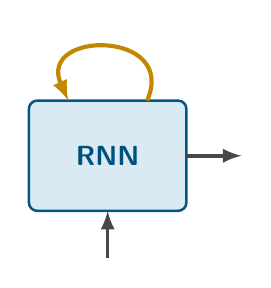
\begin{tikzpicture}[line width=0.9pt]
  \filldraw[draw=otblue!75!black, fill=otblue!15, rounded corners=3pt] (0,0) rectangle (2,1.4);
  \node[font=\sffamily\bfseries, text=otblue!70!black] at (1,0.7) {RNN};
  \draw[otorange!85!black, line width=1.5pt, -latex] (1.5,1.4) .. controls (1.9,2.3) and (0.1,2.3) .. (0.5,1.4);
  \draw[otgray!80!black, line width=1.3pt, -latex] (1,-0.6) -- (1,0);
  \draw[otgray!80!black, line width=1.3pt, -latex] (2,0.7) -- (2.7,0.7);
\end{tikzpicture}
\end{document}
